\documentclass[9pt,aspectratio=169,xcolor=table]{beamer}

%~~~~~~~~~~~~~~~~~~~~~~~~~~~~~~~~~~~~~~~~~~~~~~~~~~~~~~~~~~~~~~~~~~~~~~~~~~~~~~
% Use roboto Font (recommended)
\usepackage[sfdefault]{roboto}
\usepackage[utf8]{inputenc}
\usepackage[T1]{fontenc}
%~~~~~~~~~~~~~~~~~~~~~~~~~~~~~~~~~~~~~~~~~~~~~~~~~~~~~~~~~~~~~~~~~~~~~~~~~~~~~~

%~~~~~~~~~~~~~~~~~~~~~~~~~~~~~~~~~~~~~~~~~~~~~~~~~~~~~~~~~~~~~~~~~~~~~~~~~~~~~~
% Define where theme files are located. ('/styles')
\usepackage{styles/fluxmacros}
\usefolder{styles}
% Use Flux theme v0.1 beta
% Available style: asphalt, blue, red, green, gray
% The built-in "red" style is only a base; its colours are
% overridden with a graphite palette just below, after the theme loads.
\usetheme[style=red]{flux}
%~~~~~~~~~~~~~~~~~~~~~~~~~~~~~~~~~~~~~~~~~~~~~~~~~~~~~~~~~~~~~~~~~~~~~~~~~~~~~~

%~~~~~~~~~~~~~~~~~~~~~~~~~~~~~~~~~~~~~~~~~~~~~~~~~~~~~~~~~~~~~~~~~~~~~~~~~~~~~~
% SKEE1033 graphite palette override.
\definecolor{primaryLight}{HTML}{5A6068} % lighter graphite -- headers, accents
\definecolor{primary}{HTML}{3A4047}      % core graphite -- titles, block headers
\definecolor{secondary}{HTML}{3A5A6B}    % muted teal -- complementary accent
\definecolor{tertiary}{HTML}{8C6A3F}     % warm bronze -- example/third accent
%~~~~~~~~~~~~~~~~~~~~~~~~~~~~~~~~~~~~~~~~~~~~~~~~~~~~~~~~~~~~~~~~~~~~~~~~~~~~~~

%~~~~~~~~~~~~~~~~~~~~~~~~~~~~~~~~~~~~~~~~~~~~~~~~~~~~~~~~~~~~~~~~~~~~~~~~~~~~~~
% Extra packages
\usepackage{booktabs}
\usepackage{colortbl}
\usepackage{ragged2e}
\usepackage{amssymb}
\usepackage{multirow}
\usepackage{tikz}
\usetikzlibrary{arrows.meta, positioning, fit, backgrounds, calc, shapes.geometric}
\setbeamertemplate{itemize items}[square]
\usepackage[scaled=.92]{beramono}
\usepackage{listings}
\usepackage{array}
% Table striping: odd rows white, even rows very light gray.
\definecolor{stripe}{gray}{0.94}
\newcommand{\striped}{\rowcolors{1}{white}{stripe}}
%~~~~~~~~~~~~~~~~~~~~~~~~~~~~~~~~~~~~~~~~~~~~~~~~~~~~~~~~~~~~~~~~~~~~~~~~~~~~~~

%~~~~~~~~~~~~~~~~~~~~~~~~~~~~~~~~~~~~~~~~~~~~~~~~~~~~~~~~~~~~~~~~~~~~~~~~~~~~~~
% Code listing style (lightweight analogue of the book's skpython style).
% This course is Python-only, so Python is set as the lstlisting default via
% \lstset below -- every \begin{lstlisting} needs no language=... of its own.
\definecolor{codebg}{HTML}{1E1E2A}
\definecolor{codetext}{HTML}{E6E6E6}
\definecolor{codegreen}{HTML}{6A9955}
\definecolor{codestring}{HTML}{D7BA3A}
\definecolor{codekeyword}{HTML}{4FA3F7}
\lstdefinestyle{skpython}{
    basicstyle=\ttfamily\footnotesize\color{codetext},
    keywordstyle=\color{codekeyword}\bfseries,
    commentstyle=\itshape\color{codegreen},
    stringstyle=\ttfamily\color{codestring},
    backgroundcolor=\color{codebg},
    breaklines=true,
    keepspaces=true,
    showspaces=false,
    showstringspaces=false,
    frame=none,
    numbers=none,
}
\lstset{language=Python, style=skpython}
%~~~~~~~~~~~~~~~~~~~~~~~~~~~~~~~~~~~~~~~~~~~~~~~~~~~~~~~~~~~~~~~~~~~~~~~~~~~~~~

%~~~~~~~~~~~~~~~~~~~~~~~~~~~~~~~~~~~~~~~~~~~~~~~~~~~~~~~~~~~~~~~~~~~~~~~~~~~~~~
% TikZ block styles for the computation-cycle and control-structure diagrams
\definecolor{cycfill}{HTML}{F3DCE4}
\definecolor{cycline}{HTML}{3A4047}
\definecolor{cycdofill}{HTML}{E8EEF0}
\definecolor{cycdoline}{HTML}{3A5A6B}
\tikzset{
  cycstep/.style = {font=\sffamily\small, align=center, rounded corners=2pt,
                     draw=cycline, fill=cycfill, line width=0.7pt,
                     minimum height=7mm, minimum width=20mm, inner sep=3pt},
  cycdo/.style   = {cycstep, fill=cycdofill, draw=cycdoline},
  flow/.style    = {-{Stealth[length=2mm]}, thick, draw=cycline},
}
%~~~~~~~~~~~~~~~~~~~~~~~~~~~~~~~~~~~~~~~~~~~~~~~~~~~~~~~~~~~~~~~~~~~~~~~~~~~~~~

%%%%%%%%%%%%%%%%%%%%%%%%%%%%%%%%%%%
%% SECTION SEPARATOR (ToC recap) %%
%%%%%%%%%%%%%%%%%%%%%%%%%%%%%%%%%%%
\AtBeginSection[]
{
{
    \setbeamercolor{background canvas}{bg=primaryLight!6}
    \begin{frame}[plain]
        \frametitle{Table of Contents}
        \tableofcontents[currentsection]
    \end{frame}
}
}
%%%%%%%%%%%%%%%%%%%%%%%%%%%%%%%%%%%

%~~~~~~~~~~~~~~~~~~~~~~~~~~~~~~~~~~~~~~~~~~~~~~~~~~~~~~~~~~~~~~~~~~~~~~~~~~~~~~
% Information
\title{A First Look at Machine Learning}
\subtitle{\emph{Engineering Computation with Python} --- Chapter 15}
\author{Mun\'{i}m Zabidi}
\institute{\color{primary}Faculty of Electrical Engineering, Universiti Teknologi Malaysia}
\date{\today}
\titlegraphic{assets/logoutmwhite.png}
%~~~~~~~~~~~~~~~~~~~~~~~~~~~~~~~~~~~~~~~~~~~~~~~~~~~~~~~~~~~~~~~~~~~~~~~~~~~~~~

\begin{document}

\titlepage

\begin{frame}{Table of Contents}
    \tableofcontents
\end{frame}

%===============================================================================
\section{What Is Machine Learning?}
%===============================================================================

\begin{frame}{The Computer Learns the Rule}
    \leavevmode
    \begin{alertblock}{An enrichment chapter}
        This chapter is \alert{not a separate teaching week}. It shows
        the main ideas with two very small models.
    \end{alertblock}

    \vspace{3mm}
    \begin{columns}[t]
        \begin{column}{.5\textwidth}
            \begin{block}{Traditional programming}
                \small A person writes the rule or equation that
                connects inputs to outputs.
            \end{block}
        \end{column}
        \begin{column}{.5\textwidth}
            \begin{block}{Machine learning}
                \small A model is trained on example inputs and outputs,
                and \alert{learns the rule itself}.
            \end{block}
        \end{column}
    \end{columns}
\end{frame}

\begin{frame}{Three Types of Machine Learning}
    \leavevmode
    \small
    \begin{columns}[t]
        \begin{column}{.33\textwidth}
            \begin{block}{Supervised}
                \scriptsize Learns from \alert{labelled} training data.
                \emph{E.g.} regression, classification.
            \end{block}
        \end{column}
        \begin{column}{.33\textwidth}
            \begin{block}{Unsupervised}
                \scriptsize Learns from \alert{unlabelled} data, finding
                patterns on its own.
            \end{block}
        \end{column}
        \begin{column}{.33\textwidth}
            \begin{block}{Reinforcement}
                \scriptsize Learns through \alert{feedback}, reinforcing
                correct responses.
            \end{block}
        \end{column}
    \end{columns}

    \vspace{3mm}
    {\small This chapter's examples are all \alert{supervised} ---
    regression and decision-tree classification.}
\end{frame}

\begin{frame}{The General Machine Learning Workflow}
    \leavevmode
    \begin{center}
    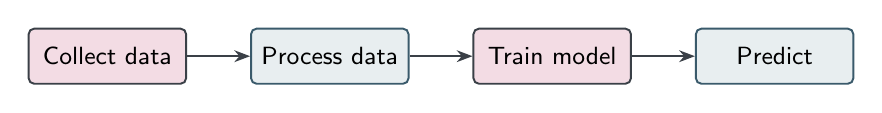
\begin{tikzpicture}[node distance=6mm and 8mm]
        \node[cycstep]                  (c) {Collect data};
        \node[cycdo, right=of c]        (p) {Process data};
        \node[cycstep, right=of p]      (t) {Train model};
        \node[cycdo, right=of t]        (u) {Predict};
        \draw[flow] (c) -- (p);
        \draw[flow] (p) -- (t);
        \draw[flow] (t) -- (u);
    \end{tikzpicture}
    \end{center}

\end{frame}

%===============================================================================
\section{Preparing Data}
%===============================================================================

\begin{frame}[fragile]{Cleaning and Scaling}
    \leavevmode
\begin{lstlisting}
import pandas as pd
from sklearn.preprocessing import StandardScaler

df = pd.DataFrame({'height': [157, 163, 176, 152, None]})
df['height'] = df['height'].fillna(df['height'].mean())   # cleaning
df['height_scaled'] = StandardScaler().fit_transform(df[['height']])
print(df)
\end{lstlisting}

    \begin{alertblock}{Fit the scaler on the training data only}
        \small When you also split the data into training and testing
        sets, fit the scaler on the \alert{training set} and use it to
        transform both. Otherwise the test set leaks into training.
    \end{alertblock}
\end{frame}

%===============================================================================
\section{Classification with a Decision Tree}
%===============================================================================

\begin{frame}{Regression vs.\ Classification}
    \leavevmode
    Predictive models divide into two kinds, by what they produce:

    \vspace{2mm}
    \begin{columns}[t]
        \begin{column}{.5\textwidth}
            \begin{block}{Regression}
                \small Predicts a \alert{quantity} --- a temperature, a
                voltage, a time constant. \\
                \emph{``How hot will this motor get?''}
            \end{block}
        \end{column}
        \begin{column}{.5\textwidth}
            \begin{block}{Classification}
                \small Predicts a \alert{category} --- healthy or
                faulty, pass or fail. \\
                \emph{``Is this motor overheating?''}
            \end{block}
        \end{column}
    \end{columns}
\end{frame}

\begin{frame}[fragile]{A Simple Decision Tree}
    \leavevmode
\begin{lstlisting}
from sklearn.tree import DecisionTreeClassifier

X = [[1], [2], [3], [4]]
y = ['low', 'low', 'high', 'high']

model = DecisionTreeClassifier()
model.fit(X, y)
print(model.predict([[3]])[0])   # high
\end{lstlisting}

    \begin{alertblock}{A model has no sense of its own limits}
        Asked to classify $99$ --- far outside its training data --- it
        still returns \texttt{high} regardless, since its only rule is
        ``above 2.5''. Judging when a question falls outside the
        model's experience remains the engineer's job.
    \end{alertblock}
\end{frame}

%===============================================================================
\section{Regression: Predicting a Quantity}
%===============================================================================

\begin{frame}[fragile]{A Straight-Line Regression}
    \leavevmode
\begin{lstlisting}
import numpy as np
from sklearn.linear_model import LinearRegression

X = np.array([26, 30, 35, 40]).reshape(-1, 1)   # temperature (C)
y = np.array([1000, 2500, 3500, 4500])          # ice-cream sales

model = LinearRegression().fit(X, y)
print(model.predict([[45]])[0])                 # 5847.62979684...
\end{lstlisting}

    \begin{alertblock}{This is an extrapolation}
        $45\,^{\circ}\text{C}$ is \alert{outside} the training range
        ($26$ to $40\,^{\circ}\text{C}$). The model just extends its
        line; nothing in the data shows that sales keep rising the same
        way. Trust it much less than a prediction inside the range.
    \end{alertblock}
\end{frame}

%===============================================================================
\section{Training and Testing Sets}
%===============================================================================

\begin{frame}[fragile]{Hold Some Data Back}
    \leavevmode
\begin{lstlisting}
from sklearn.model_selection import train_test_split
from sklearn.linear_model import LinearRegression

X = [[22], [24], [26], [28], [30], [32], [34], [36], [38], [40]]
y = [450, 700, 1000, 1700, 2500, 2800, 3300, 3700, 4100, 4500]

X_train, X_test, y_train, y_test = train_test_split(
    X, y, test_size=0.2, random_state=0)
model = LinearRegression().fit(X_train, y_train)
print(f"{model.score(X_train, y_train):.3f}")   # 0.992 (training)
print(f"{model.score(X_test, y_test):.3f}")     # 0.975 (unseen data)
\end{lstlisting}

    \begin{block}{The test score is the honest one}
        \small A large gap between the two scores is the classic sign
        of \alert{overfitting}.
    \end{block}
\end{frame}

%===============================================================================
\section{Summary}
%===============================================================================

\begin{frame}{Where This Leaves You}
    \leavevmode
    \small
    \begin{itemize}
        \item In machine learning a model \alert{learns the rule} from
              examples; this book uses only supervised learning.
        \item \texttt{DecisionTreeClassifier} predicts a category;
              \texttt{LinearRegression} predicts a number.
        \item Always judge a model on a \alert{test set} it has not
              seen, and fit any scaler on the training set only.
        \item No model can be trusted outside the range of its training
              data: machine learning is \alert{one more engineering
              tool}, not a substitute for understanding the problem.
    \end{itemize}
\end{frame}

\end{document}
